\documentclass[14pt]{extbook}
\usepackage{multicol, enumerate, enumitem, hyperref, color, soul, setspace, parskip, fancyhdr} %General Packages
\usepackage{amssymb, amsthm, amsmath, latexsym, units, mathtools} %Math Packages
\everymath{\displaystyle} %All math in Display Style
% Packages with additional options
\usepackage[headsep=0.5cm,headheight=12pt, left=1 in,right= 1 in,top= 1 in,bottom= 1 in]{geometry}
\usepackage[usenames,dvipsnames]{xcolor}
\usepackage{dashrule}  % Package to use the command below to create lines between items
\newcommand{\litem}[1]{\item#1\hspace*{-1cm}\rule{\textwidth}{0.4pt}}
\pagestyle{fancy}
\lhead{Makeup Progress Quiz 2}
\chead{}
\rhead{Version C}
\lfoot{5763-3522}
\cfoot{}
\rfoot{Spring 2021}
\begin{document}

\begin{enumerate}
\litem{
Determine the horizontal and/or oblique asymptotes in the rational function below.\[ f(x) = \frac{6x^{3} +23 x^{2} +9 x -18}{2x^{2} +9 x + 9} \]\begin{enumerate}[label=\Alph*.]
\item \( \text{Oblique Asymptote of } y = 3x -2. \)
\item \( \text{Horizontal Asymptote of } y = 3.0  \)
\item \( \text{Horizontal Asymptote at } y = -3.0 \)
\item \( \text{Horizontal Asymptote of } y = 3.0 \text{ and Oblique Asymptote of } y = 3x -2 \)
\item \( \text{Horizontal Asymptote of } y = -3.0 \text{ and Oblique Asymptote of } y = 3x -2 \)

\end{enumerate} }
\litem{
Determine the vertical asymptotes and holes in the rational function below.\[ f(x) = \frac{6x^{3} -5 x^{2} -61 x -60}{8x^{2} +2 x -15} \]\begin{enumerate}[label=\Alph*.]
\item \( \text{Vertical Asymptote of } x = 1.25 \text{ and hole at } x = -1.5 \)
\item \( \text{Vertical Asymptotes of } x = 1.25 \text{ and } x = -1.5 \text{ with no holes.} \)
\item \( \text{Vertical Asymptotes of } x = 1.25 \text{ and } x = -1.667 \text{ with a hole at } x = -1.5 \)
\item \( \text{Holes at } x = 1.25 \text{ and } x = -1.5 \text{ with no vertical asymptotes.} \)
\item \( \text{Vertical Asymptote of } x = 0.75 \text{ and hole at } x = -1.5 \)

\end{enumerate} }
\litem{
Which of the following functions \textit{could} be the graph below?
\begin{center}
    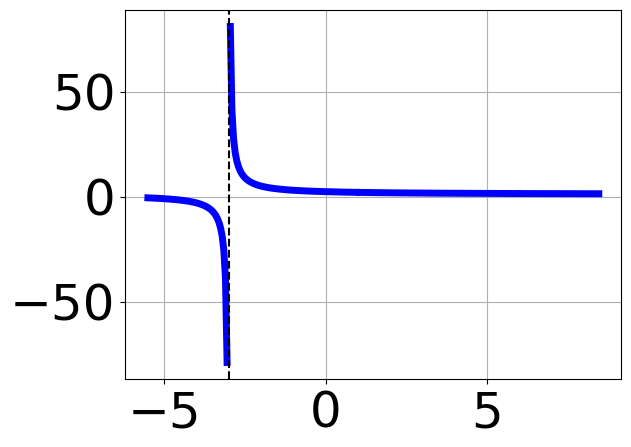
\includegraphics[width=0.5\textwidth]{../Figures/identifyGraphOfRationalFunctionCopyC.png}
\end{center}
\begin{enumerate}[label=\Alph*.]
\item \( f(x)=\frac{x^{3} -43 x + 42}{x^{3} -4 x^{2} -15 x + 18} \)
\item \( f(x)=\frac{x^{3} + x^{2} -34 x + 56}{x^{3} -4 x^{2} -15 x + 18} \)
\item \( f(x)=\frac{x^{3} -43 x -42}{x^{3} +4 x^{2} -15 x -18} \)
\item \( f(x)=\frac{x^{3} -43 x -42}{x^{3} +4 x^{2} -15 x -18} \)
\item \( \text{None of the above are possible equations for the graph.} \)

\end{enumerate} }
\litem{
Determine the horizontal and/or oblique asymptotes in the rational function below.\[ f(x) = \frac{12x^{3} -17 x^{2} -104 x -80}{3x^{2} -8 x -16} \]\begin{enumerate}[label=\Alph*.]
\item \( \text{Horizontal Asymptote of } y = 4.0 \text{ and Oblique Asymptote of } y = 4x + 5 \)
\item \( \text{Horizontal Asymptote of } y = 4.0  \)
\item \( \text{Oblique Asymptote of } y = 4x + 5. \)
\item \( \text{Horizontal Asymptote at } y = 4.0 \)
\item \( \text{Horizontal Asymptote of } y = 4.0 \text{ and Oblique Asymptote of } y = 4x + 5 \)

\end{enumerate} }
\litem{
Determine the vertical asymptotes and holes in the rational function below.\[ f(x) = \frac{12x^{3} +41 x^{2} -38 x -40}{9x^{2} +21 x + 10} \]\begin{enumerate}[label=\Alph*.]
\item \( \text{Vertical Asymptote of } x = -1.667 \text{ and hole at } x = -0.667 \)
\item \( \text{Vertical Asymptotes of } x = -1.667 \text{ and } x = 1.25 \text{ with a hole at } x = -0.667 \)
\item \( \text{Holes at } x = -1.667 \text{ and } x = -0.667 \text{ with no vertical asymptotes.} \)
\item \( \text{Vertical Asymptotes of } x = -1.667 \text{ and } x = -0.667 \text{ with no holes.} \)
\item \( \text{Vertical Asymptote of } x = 1.333 \text{ and hole at } x = -0.667 \)

\end{enumerate} }
\litem{
Determine the horizontal and/or oblique asymptotes in the rational function below.\[ f(x) = \frac{20x^{3} -13 x^{2} -23 x + 10}{-20x^{3} +66 x^{2} +21 x -20} \]\begin{enumerate}[label=\Alph*.]
\item \( \text{Horizontal Asymptote of } y = 0  \)
\item \( \text{None of the above} \)
\item \( \text{Vertical Asymptote of } y = -1  \)
\item \( \text{Vertical Asymptote of } y = 0.800  \)
\item \( \text{Horizontal Asymptote of } y = -1.000  \)

\end{enumerate} }
\litem{
Determine the vertical asymptotes and holes in the rational function below.\[ f(x) = \frac{9x^{3} +54 x^{2} +80 x + 32}{9x^{2} -16} \]\begin{enumerate}[label=\Alph*.]
\item \( \text{Vertical Asymptote of } x = 1.0 \text{ and hole at } x = -1.333 \)
\item \( \text{Vertical Asymptote of } x = 1.333 \text{ and hole at } x = -1.333 \)
\item \( \text{Vertical Asymptotes of } x = 1.333 \text{ and } x = -1.333 \text{ with no holes.} \)
\item \( \text{Vertical Asymptotes of } x = 1.333 \text{ and } x = -0.667 \text{ with a hole at } x = -1.333 \)
\item \( \text{Holes at } x = 1.333 \text{ and } x = -1.333 \text{ with no vertical asymptotes.} \)

\end{enumerate} }
\litem{
Determine the vertical asymptotes and holes in the rational function below.\[ f(x) = \frac{12x^{3} +37 x^{2} -59 x -60}{6x^{2} -19 x + 15} \]\begin{enumerate}[label=\Alph*.]
\item \( \text{Holes at } x = 1.5 \text{ and } x = 1.667 \text{ with no vertical asymptotes.} \)
\item \( \text{Vertical Asymptotes of } x = 1.5 \text{ and } x = -0.75 \text{ with a hole at } x = 1.667 \)
\item \( \text{Vertical Asymptote of } x = 2.0 \text{ and hole at } x = 1.667 \)
\item \( \text{Vertical Asymptotes of } x = 1.5 \text{ and } x = 1.667 \text{ with no holes.} \)
\item \( \text{Vertical Asymptote of } x = 1.5 \text{ and hole at } x = 1.667 \)

\end{enumerate} }
\litem{
Which of the following functions \textit{could} be the graph below?
\begin{center}
    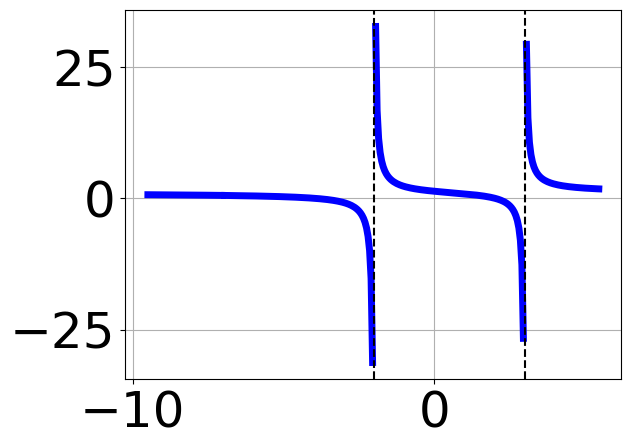
\includegraphics[width=0.5\textwidth]{../Figures/identifyGraphOfRationalFunctionC.png}
\end{center}
\begin{enumerate}[label=\Alph*.]
\item \( f(x)=\frac{x^{3} -9 x^{2} +6 x + 56}{x^{3} -6 x^{2} -13 x + 42} \)
\item \( f(x)=\frac{x^{3} -2 x^{2} -16 x + 32}{x^{3} +6 x^{2} -13 x -42} \)
\item \( f(x)=\frac{x^{3} -9 x^{2} +6 x + 56}{x^{3} -6 x^{2} -13 x + 42} \)
\item \( f(x)=\frac{x^{3} +9 x^{2} +6 x -56}{x^{3} +6 x^{2} -13 x -42} \)
\item \( \text{None of the above are possible equations for the graph.} \)

\end{enumerate} }
\litem{
Determine the horizontal and/or oblique asymptotes in the rational function below.\[ f(x) = \frac{18x^{3} +81 x^{2} +16 x -80}{12x^{3} -50 x^{2} -135 x + 100} \]\begin{enumerate}[label=\Alph*.]
\item \( \text{None of the above} \)
\item \( \text{Vertical Asymptote of } y = 2.500  \)
\item \( \text{Vertical Asymptote of } y = -4  \)
\item \( \text{Horizontal Asymptote of } y = 1.500  \)
\item \( \text{Horizontal Asymptote of } y = 0  \)

\end{enumerate} }
\end{enumerate}

\end{document}